\section{Alloy}
\lstset{
  language=alloy,
  basicstyle=\small\ttfamily,
  breaklines=true,
  showstringspaces=false
}
In this section it is provided a representation of the world of CKB using the Alloy language. Every run and every check are commented in order to guarantee a syntactical correct compilation of the code: it is up to the reader to decide what to uncomment based on their will.

\lstinputlisting{4Alloy/res/third_model.als}

\subsection{Generated World}
\begin{figure}[h]
  \centering
  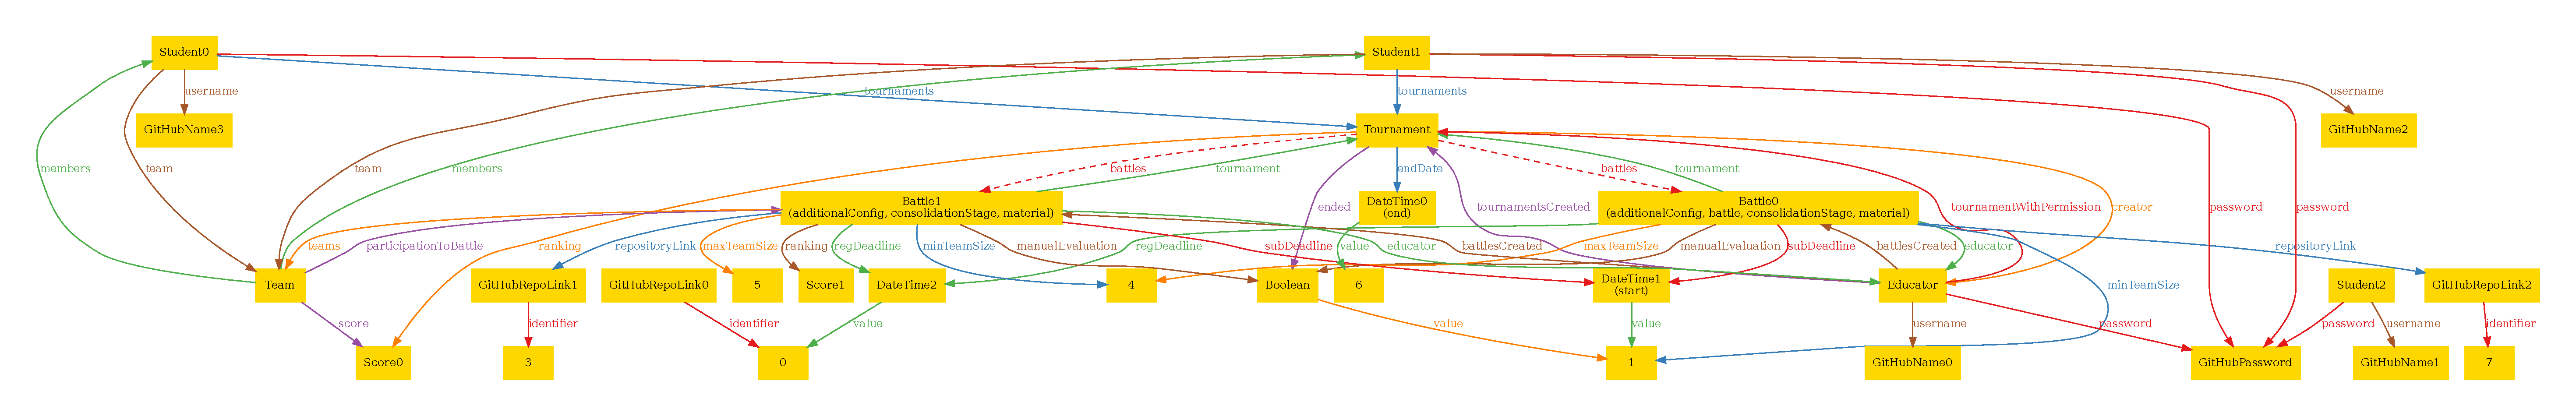
\includegraphics[width=1.1\linewidth]{4Alloy/res/general.pdf}
  \caption{The world generated by running \textit{general} predicate projected over nine signatures (ABS, CodeTest, ConsolidationStage, Description, EducatorMaterial, EvaluationCriteria, Macrovariables, Notification, String) in order to be more comprehensible. This world represents a normal situation of the model}
\end{figure}

\begin{figure}[h]
  \centering
  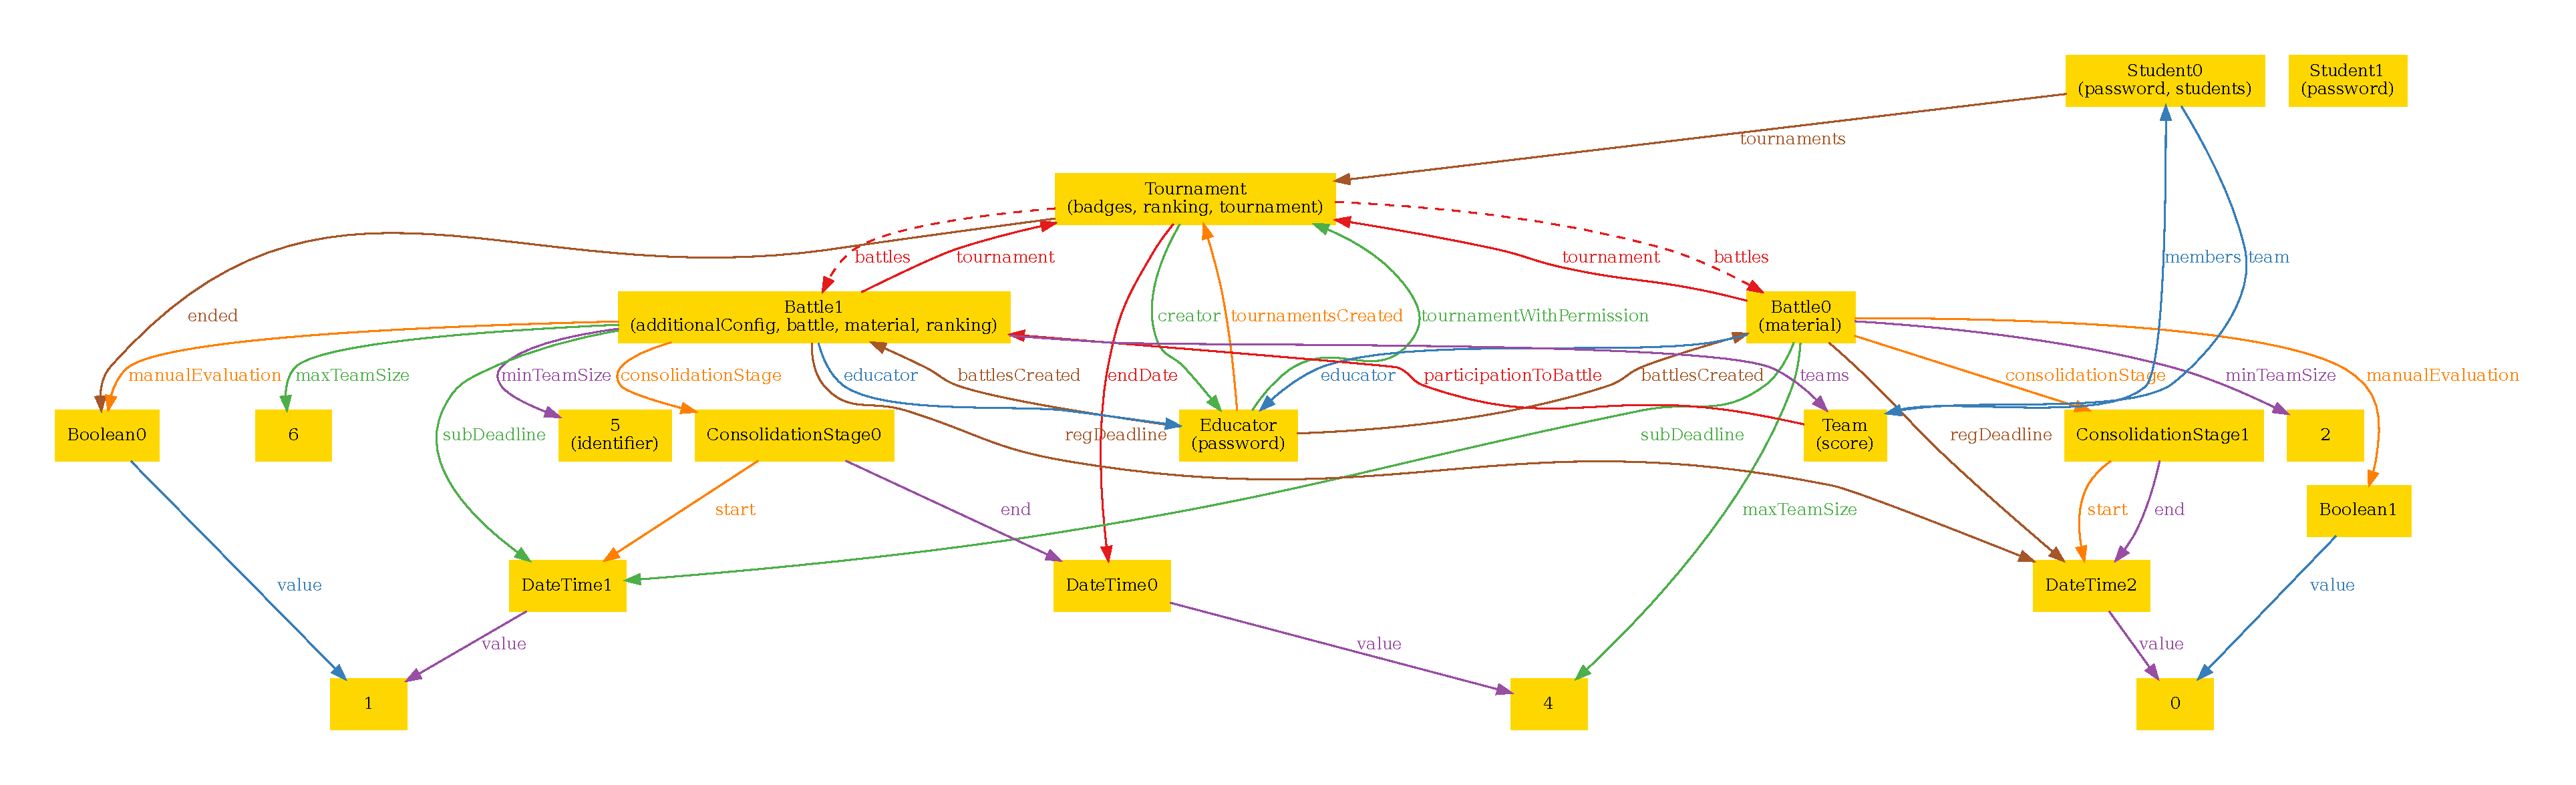
\includegraphics[width=1.1\linewidth]{4Alloy/res/noManualEvaluation.pdf}
  \caption{The world generated by running \textit{noManualEvaluation} predicate projected over thirteen signatures (ABS, Badge, CodeTest, Description, EducatorMaterial, EvaluationCriteria, GitHubName, GitHubPassword, GitHubRepoLink, Macrovariables, Notification, Score, String) in order to be more comprehensible. This world represents the situation where there is no manual evaluation for one battle out of two. It is useful in order to see the right aim of the model. Indeed, as you can see, in the case the manualEvaluation is not required (the boolean value equals 0) there is no consolidation stage, and viceversa}
\end{figure}

\afterpage{
  \clearpage
  \begin{figure}[h]
  \centering
  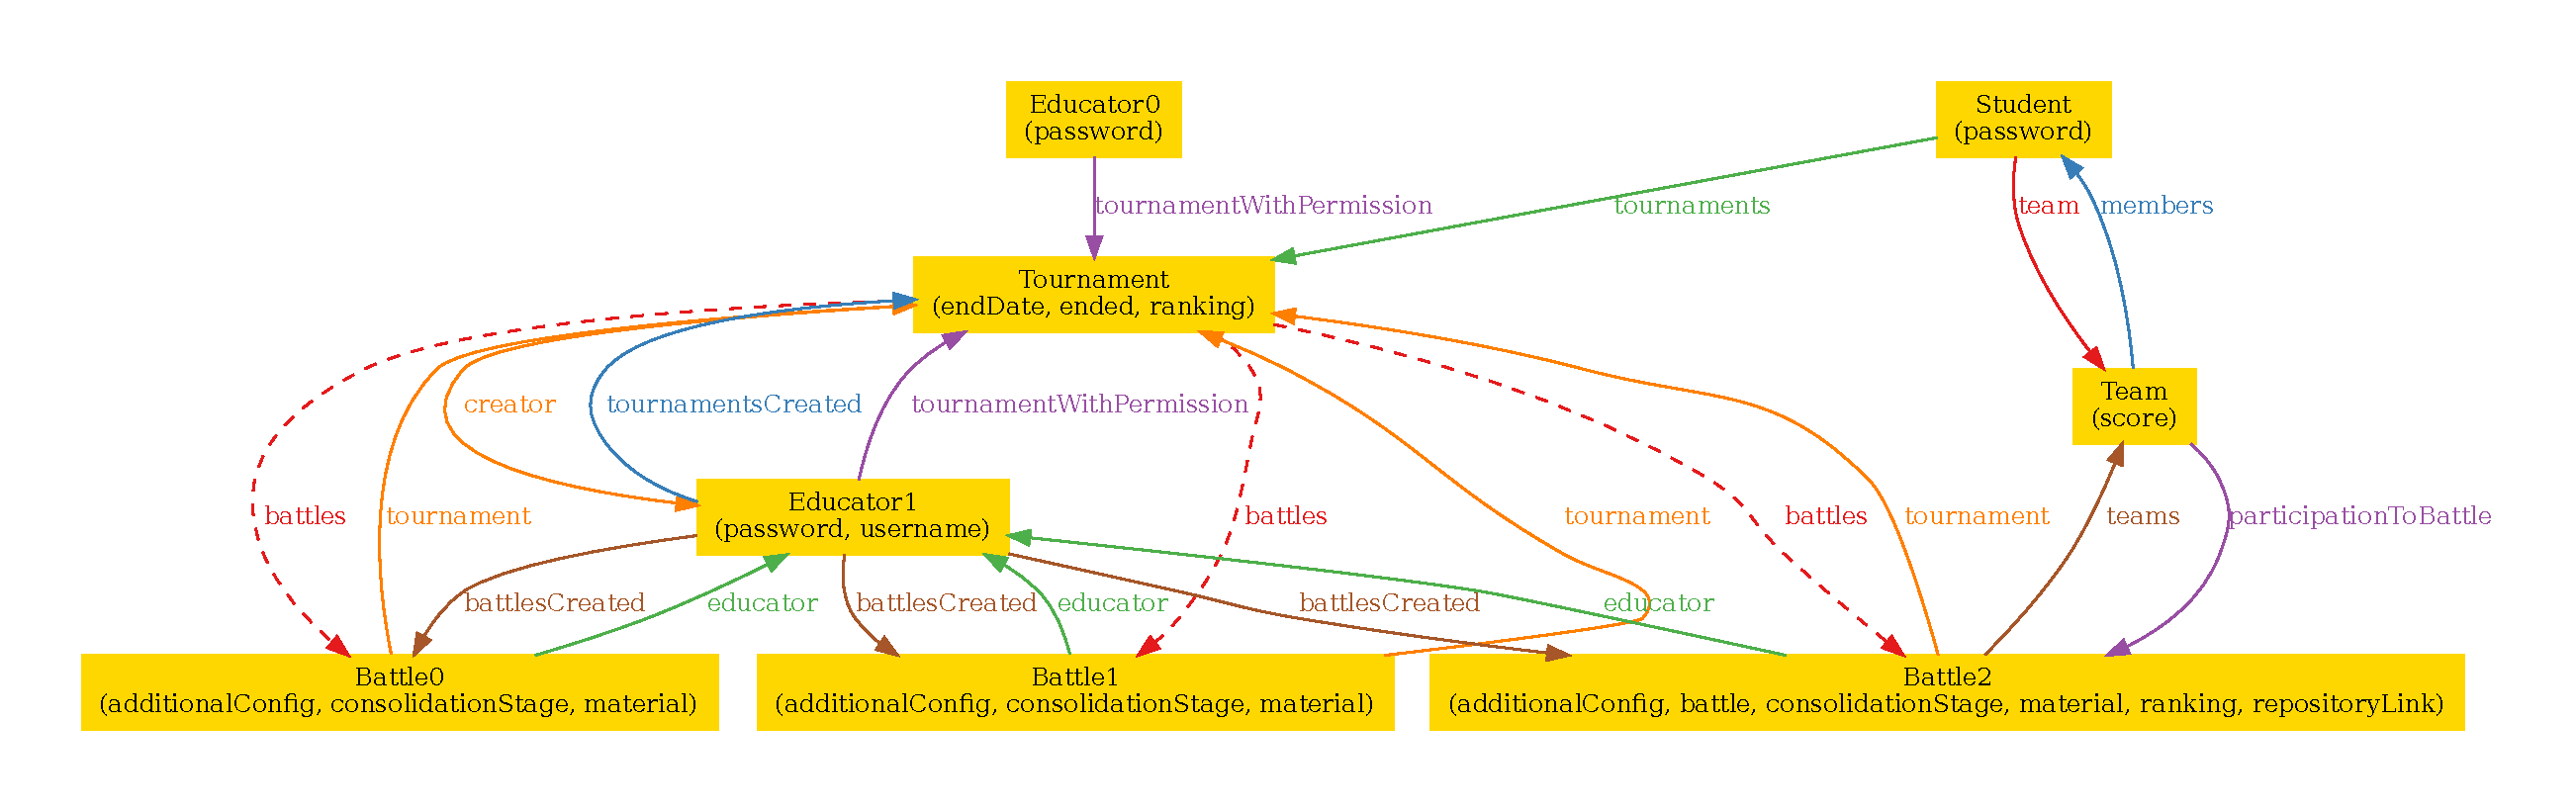
\includegraphics[angle=90, width=0.3\textwidth, height=1.35\textwidth]{RASD/4Alloy/res/educatorsWithOnlyPermission.pdf}
  \label{fig:educatorsWithOnlyPermission_alloy}
  \newpage
  \end{figure}
  \clearpage 
  \captionof{figure}{The world generated by running \textit{educatorsWithOnlyPermission} projected over seventeen signatures (ABS, Badge, Boolean, CodeTest, ConsolidationStage, DateTime, Description, EducatorMaterial, EvaluationCriteria, GitHubName, GitHubPassword, GitHubRepoLink, Int, Macrovariables, Notification, Score, String) in order to be more comprehensible. This world represents the situation where there are educator with permissions for a tournament they haven't created. As you can see, it cannot exist a tournament without a creator, but some educators can have tournaments with only the permission, without having created them}
}



